\chapter{Conditional Wasserstein GAN}

In this chapter, we introduce the Conditional Wasserstein Generative Adversarial Network (CWGAN) architecture,
which extends the traditional conditional GAN framework by means of the Wasserstein distance exploitation.\\

The main changes that characterize the CWGAN with respect to the CGAN are:
\begin{itemize}
    \item The loss function of a standard GAN is based on Jensen-Shannon divergence minimization while the CWGAN is based on the Wasserstein distance, which provides a more stable training process and mitigates issues such as mode collapse.
    \item The discriminator, which in Wasserstein GAN architecture is called critic, is designed to output real-valued scores instead of probabilities, allowing it to better capture the differences between real and generated data distributions.
    For this reason, the discriminator network does not use a sigmoid activation function in the output layer.
    \item The training procedure requires as a good practice to optimize the critic multiple times per generator update to ensure that the critic provides accurate gradients for the generator.
    \item The use of gradient penalty term in the loss function has the objective to enforce the Lipschitz constraint required for the Wasserstein distance computation.  
\end{itemize}


Now the critic maximizes the following loss function $E_{\boldsymbol{x} \sim p_d}[D(\boldsymbol{x})]-E_{\widehat{\boldsymbol{x}} \sim p_g}[D(\widehat{\boldsymbol{x}})]$ where $\boldsymbol{x}$ are real data samples from the data distribution $p_d$ and $\widehat{\boldsymbol{x}}$ are generated samples from the generator distribution $p_g$.
On the other hand, the generator minimizes the loss function $-E_{\widehat{\boldsymbol{x}} \sim p_g}[D(\widehat{\boldsymbol{x}})]$.\\
Given this setup, there is no need anymore for true and fake data labels since the critic outputs real-valued scores.\\
An additional advatage of using the Wasserstein distance is that it provides a meaningful measure of the distance between the real and generated data distributions, which allows for the implementation of an early stopping technique which
improve the training efficiency.\\

\section{Experiment results}
In this section, we present the results obtained from training the CWGAN architecture on the same dataset used for the CGAN experiments, 
by following the same data simulation, preprocessing, and evaluation procedures described before.\\



\begin{figure}[H]
    \centering
    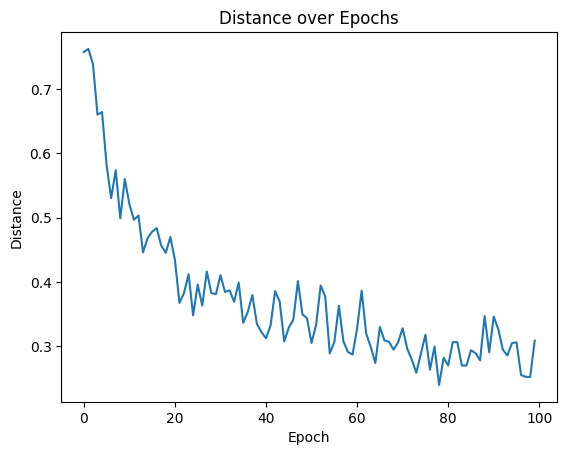
\includegraphics[width=0.9\textwidth]{Background2/images/CWGAN_learning_curve.png}
    \caption{Distance between real and generated probability density function of the standard normal distribution over epochs.}
    \label{cwgan_global_error}
\end{figure}



\begin{figure}[H]
    \centering
    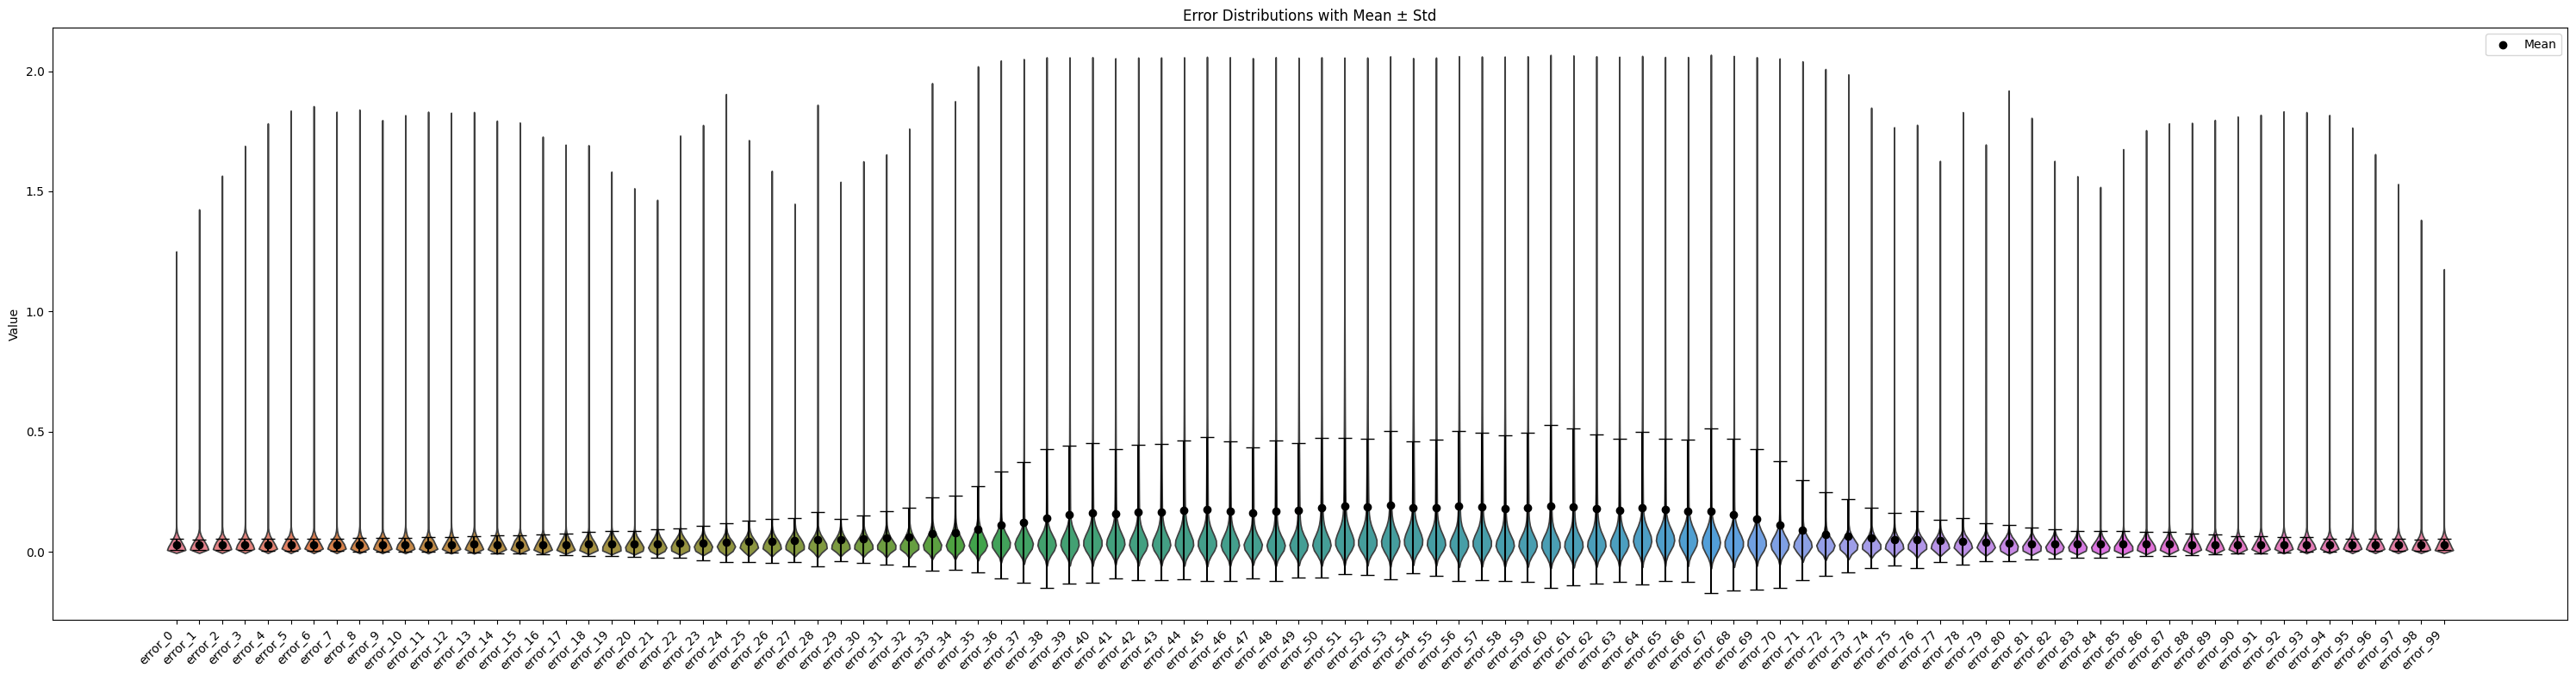
\includegraphics[width=1.0\textwidth]{Background2/images/CWGAN_error_dist.png}
    \caption{Error distribution between real and generated bins probabilities using global bins.}
    \label{cwgan_global_error}
\end{figure}



\begin{figure}[H]
    \centering
    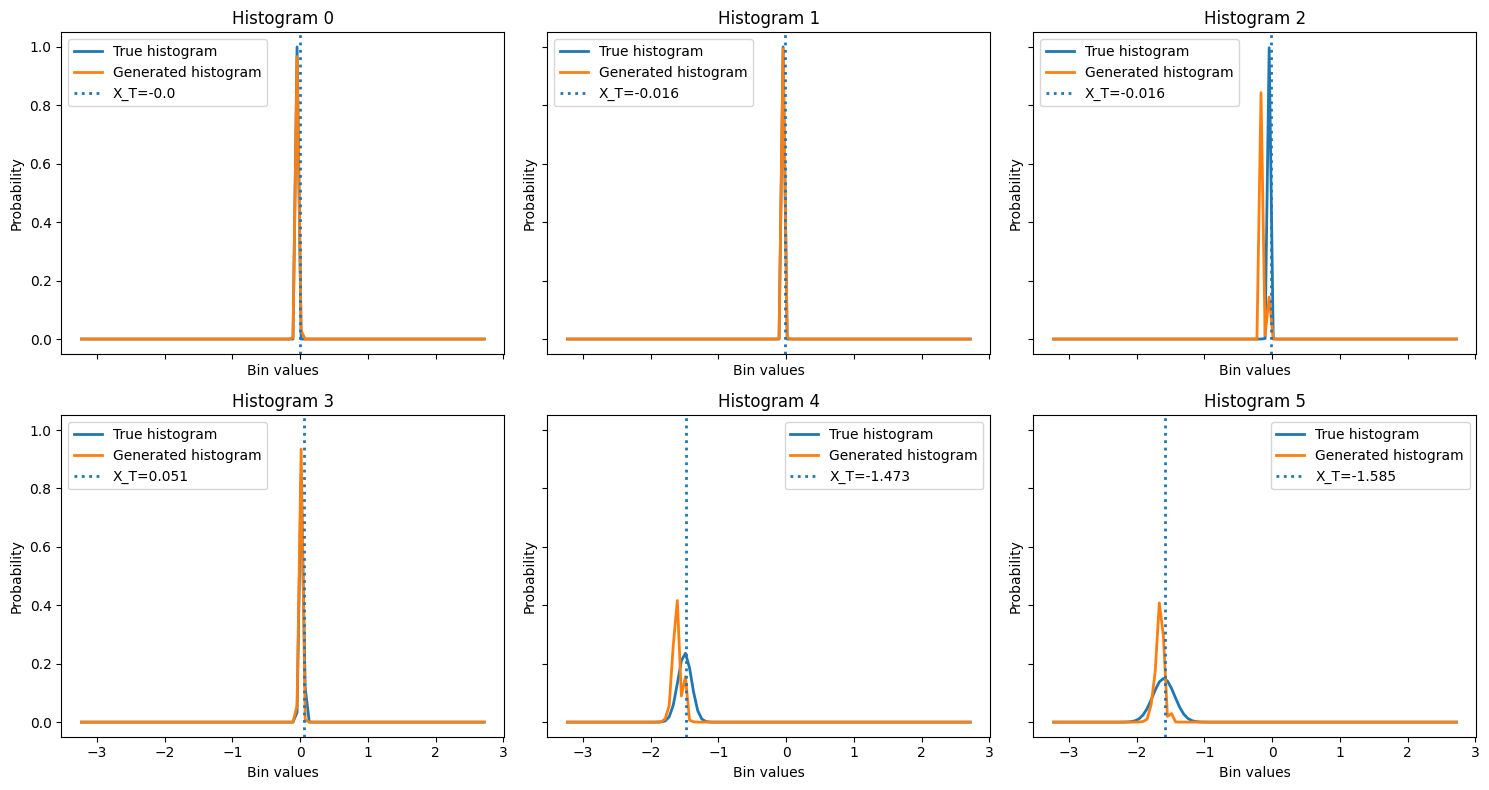
\includegraphics[width=1.0\textwidth]{Background2/images/CWGAN_bins_samples_v2.png}
    \caption{Samples obtained using fixed $X_0$ and $\mu$ while varying $\sigma = [0.001, 0.01, 0.05, 0.1, 0.5, 0.8]$.}
    \label{cwgan_sample_sigma}
\end{figure}


As can be seen from \ref{cwgan_sample_sigma} the quality of the generated distributions is significantly improved with respect to the CGAN results shown in \ref{bins_global_sample_sigma}.
This is also confirmed by running the Kolmogorov-Smirnov test over 1000 generated samples. The results show that
30\% of the generated samples are accepted at a significance level of 1\%, compared to only 2.5\% acceptance rate for the CGAN model.\\
However, the model is still not perfect since for higher values of $\sigma$ the generated distributions still deviate from the real ones.
Further hyperparameter tuning and model architecture adjustments may be necessary to achieve better performance.

